%----------------------------------------------------------------------------------------
% Contenido del Informe - Resultados
%----------------------------------------------------------------------------------------

\chapter{Resultados}

\section{Puntos 1 y 2}

A continuación se mostrarán los gráficos obtenidos de los puntos 1 y 2:

\begin{figure}[H]
	\centering
	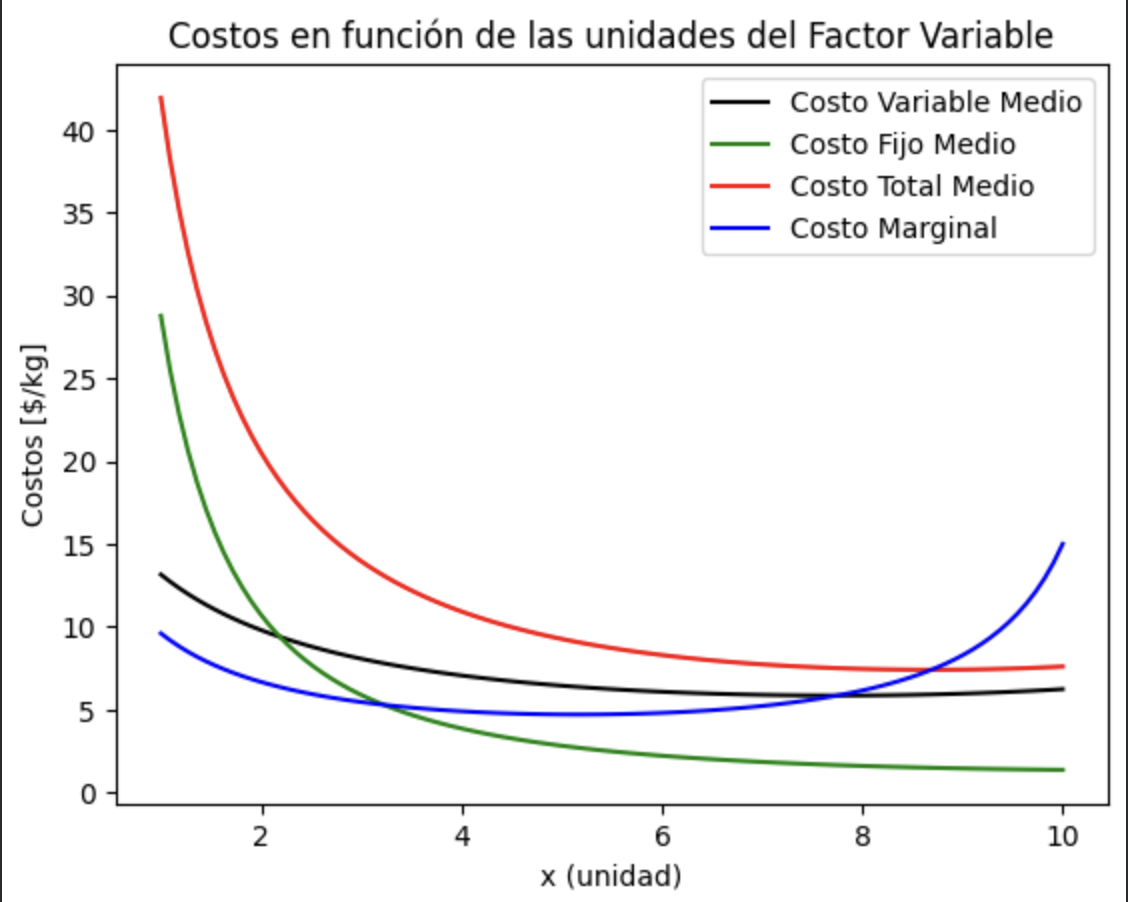
\includegraphics[width=0.8\textwidth]{imagenes/costo.factor.var.png}
	\caption{Costos en función de las unidades de factor variable}
\end{figure}

\begin{figure}[H]
	\centering
	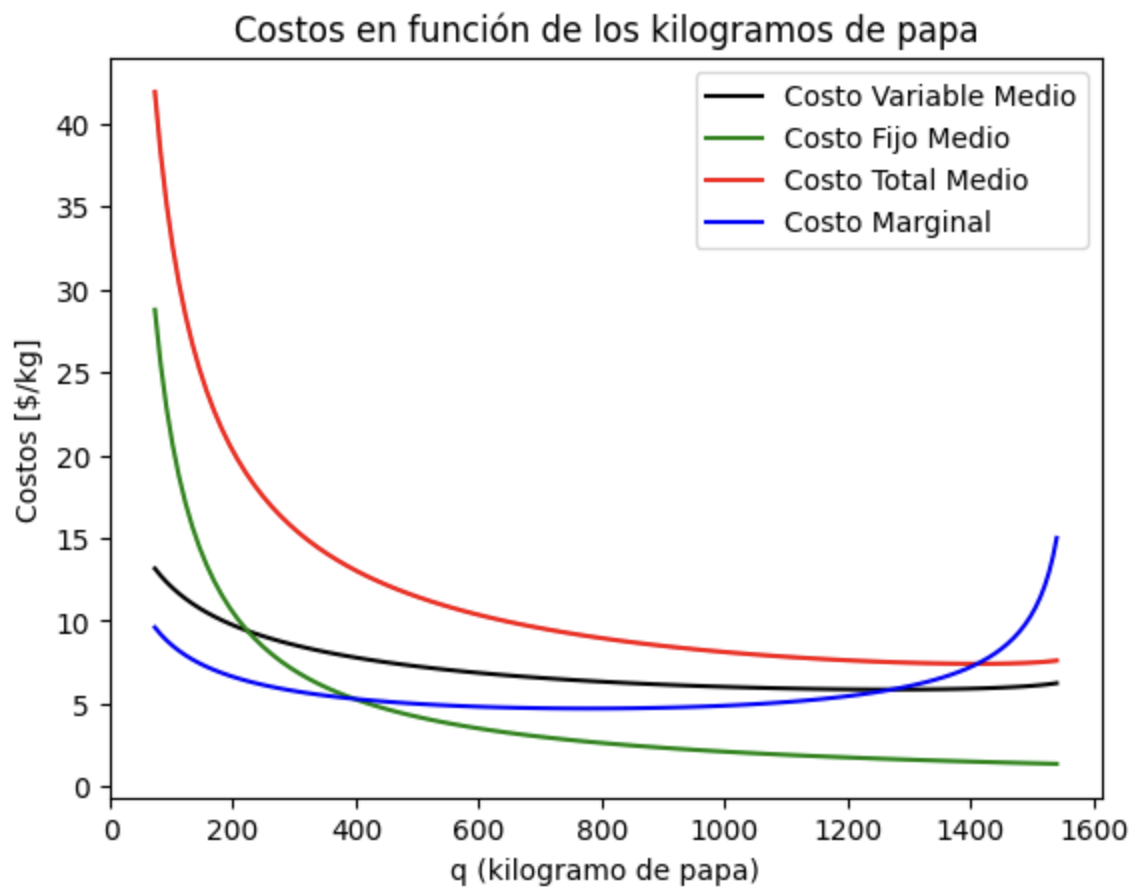
\includegraphics[width=0.8\textwidth]{imagenes/costo.kg.png}
	\caption{Costos en función de los kg de papa}
\end{figure}

\begin{figure}[H]
	\centering
	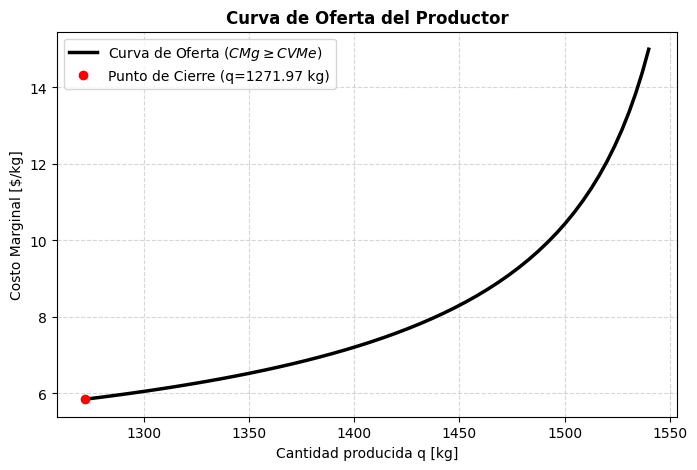
\includegraphics[width=0.8\textwidth]{imagenes/c.oferta.nueva.png}
	\caption{Curva de la oferta}
\end{figure}


Se muestra la tabla correspondiente a las raíces de funciones calculadas:

\begin{table}[htbp]
\centering
\resizebox{\textwidth}{!}{
\begin{tabular}{ccccccccc}
\toprule
\textbf{Paso (i)} & \textbf{xi} & \textbf{f(xi)} & \textbf{f'(xi)} & \textbf{x(i+1)} & \textbf{Error abs} & \textbf{Dec. sig} & \textbf{Error rel} & \textbf{Cifras sig} \\
\midrule
0 & 8.000000 & 8.000000 & 33.000000 & 7.757576 & 0.242424 & 0.000000 & 0.031250 & 2.000000 \\
1 & 7.757576 & 0.235078 & 31.060606 & 7.750007 & 0.007568 & 1.000000 & 0.000977 & 3.000000 \\
2 & 7.750007 & 0.000229 & 31.000059 & 7.750000 & 0.000007 & 4.000000 & 0.000001 & 6.000000 \\
\bottomrule
\end{tabular}
}
\caption{Tabla Punto 2}
\label{tab:punto2}
\end{table}



El resultado que se obtiene mediante este método se lo compara con la raíz exacta: $4x^3 = 31x^2$, que si se resuelve de forma analítica da dos raíces: $x = 7,75$, la cual está dentro del rango solicitado y coincide con precisión matemática con la obtenida mediante el método numérico; y $x = 0$, que al encontrarse fuera del rango de estudio se descarta.






\section{Punto 3}

Se presenta la evolución iterativa para la determinación del nivel óptimo de factor variable a partir de la condición de maximización del beneficio ($B'(x) = 0$). La resolución numérica mediante el método de Newton-Raphson se detalla en la Tabla \ref{tab:punto3}.

\begin{table}[htbp]
\centering
\resizebox{\textwidth}{!}{
    \begin{tabular}{lrrrrrrrr}
\toprule
 & xi & f(xi) & f'(xi) & x(i+1) & Error abs & Decimales sig & Error rel & Cifras sig \\
Paso (i) &  &  &  &  &  &  &  &  \\
\midrule
0 & 9.000000 & 200.000000 & -460.000000 & 9.434783 & 0.434783 & 0.000000 & 0.046083 & 2.000000 \\
1 & 9.434783 & -11.342155 & -512.173913 & 9.412637 & 0.022145 & 1.000000 & 0.002353 & 3.000000 \\
2 & 9.412637 & -0.029424 & -509.516498 & 9.412580 & 0.000058 & 3.000000 & 0.000006 & 5.000000 \\
3 & 9.412580 & -0.000000 & -509.509568 & 9.412580 & 0.000000 & 9.000000 & 0.000000 & 11.000000 \\
\bottomrule
\end{tabular}
}
    \caption{Resultado raíz punto 3 por el método de Newton-Raphson.}
    \label{tab:punto3}
\end{table}

Para validar la precisión del algoritmo, se contrasta el valor numérico obtenido con la resolución de la raíz exacta del modelo analítico:
\begin{equation} 
x = \dfrac{31}{6} \pm \dfrac{\sqrt{745-24N}}{6} 
\end{equation} 

Al reemplazar por el parámetro económico $N = 4$ asignado a nuestro grupo, se obtienen las siguientes soluciones teóricas:
\begin{itemize}
    \item $x_{1} = 9,41258$: Valor óptimo que se localiza dentro del rango operativo y técnico de producción solicitado $[1; 10]$.
    \item $x_{2} = 0,92075$: Valor que se ubica por debajo del punto de cierre biológico y económico de la firma, motivo por el cual se descarta al no representar una operación sustentable.
\end{itemize}

A partir de la raíz válida truncada a seis cifras significativas ($x = 9,41258$), se evalúa de forma analítica el beneficio económico de la firma mediante la ecuación:
\begin{equation}
Beneficio = (44 \cdot 9,41258 + 31 \cdot 9,41258^2 - 2 \cdot 9,41258^3) \cdot 10 - (960 \cdot 9,41258 + 2100)
\end{equation}

El desglose aritmético en papel de los componentes del ingreso y del costo total bajo este criterio de redondeo manual arroja:
\begin{itemize}
    \item Producción obtenida ($q$): $1385,849$ kg de papa.
    \item Ingreso Total ($IT$): $13858,49$ \$.
    \item Costo Total ($CT$): $9036,08 + 2100 = 11136,08$ \$.
    \item \textbf{Beneficio analítico en papel = 2722,41 \ \$}
\end{itemize}

Es fundamental destacar que la evaluación algorítmica automatizada directa dentro del cuaderno de Colab arroja un valor final de \textbf{\$3791,96}. Esta discrepancia numérica no constituye un error conceptual ni un fallo en el entorno programado, sino que responde de manera exclusiva al fenómeno de propagación de errores por redondeo. Mientras que el cálculo manuscrito introduce una aproximación al fijar la raíz en cinco decimales, el procesador de la computadora conserva la precisión en punto flotante completa de la variable en memoria. Al verse afectados por el exponente cúbico de la función de producción de papa ($-2x^3$), estos decimales residuales se amplifican significativamente, justificando la diferencia observada y validando el rigor computacional del script frente al cálculo teórico acotado.







\section{Punto 4}

Se expone el proceso iterativo del método de Newton-Raphson aplicado para hallar el nivel de factor variable que garantiza un beneficio del 15\% sobre el costo total, el cual exige cumplir la condición de equilibrio $CM_e(x) = 0,85 \cdot CM_g(x)$. La convergencia digital se detalla en la Tabla \ref{tab:punto4}.

\begin{table}[htbp]
\centering
\resizebox{\textwidth}{!}{
\begin{tabular}{lrrrrrrrr}
\toprule
 & xi & f(xi) & f'(xi) & x(i+1) & Error abs & Decimales sig & Error rel & Cifras sig \\
Paso (i) &  &  &  &  &  &  &  &  \\
\midrule
0 & 9.000000 & 13650.000000 & 465600.000000 & 8.970683 & 0.029317 & 1.000000 & 0.003268 & 3.000000 \\
1 & 8.970683 & 76.772771 & 460366.274239 & 8.970516 & 0.000167 & 3.000000 & 0.000019 & 5.000000 \\
2 & 8.970516 & 0.002477 & 460336.566559 & 8.970516 & 0.000000 & 7.000000 & 0.000000 & 9.000000 \\
\bottomrule
\end{tabular}
}
    \caption{Evolución iterativa del Punto 4 por el método de Newton-Raphson.}
    \label{tab:punto4}
\end{table}

A partir de la raíz obtenida y corregida bajo los parámetros analíticos de nuestro grupo, se adopta para el desarrollo escrito el valor redondeado a seis cifras significativas ($x = 8,97052$). Evaluando dicho umbral operativo en la función de Costo Marginal, se determina el precio mínimo por kilogramo en el mercado:
\begin{equation}
\textbf{Precio por kg} = Costo \ Marginal = \dfrac{960}{44 + 62 \cdot 8,97052 - 6 \cdot 8,97052^2} = \textbf{8,21217}
\end{equation}

Multiplicando este valor unitario teórico por el kilaje comercial de la presentación estándar de la firma, se arriba al valor de la bolsa en papel:
\begin{equation}
\textbf{Precio de la bolsa (24kg)} = Precio \ por \ kg \cdot 24 = 8,21217 \cdot 24 = \textbf{197,09}
\end{equation}

Es imperativo explicitar que, al ejecutar la celda de cálculo final de forma automatizada dentro de la notebook de Colab, la consola arroja un precio de equilibrio de \textbf{\$196,33}. Al igual que en el análisis de beneficios del punto anterior, esta sutil variación responde de manera exclusiva a la tolerancia implícita y a la precisión de la máquina. Mientras el desarrollo manuscrito introduce un error de truncamiento al fijar la variable en $8,97052$, el entorno de programación evalúa el Costo Marginal utilizando la raíz nativa con punto flotante completo ($8,970516...$). Al verse afectado por la naturaleza no lineal del denominador cuadrático, este residuo infinitesimal se propaga, justificando de forma analítica y válida la diferencia de centavos entre el cálculo teórico acotado y la simulación digital.




\section{Punto 5}

Se muestra la tabla correspondiente a las raíces de funciones calculadas:

\begin{table}[htbp]
\centering
\resizebox{\textwidth}{!}{%
\begin{tabular}{lrrrrrrrr}
\toprule
 & xi & f(xi) & f'(xi) & x(i+1) & Error abs & Decimales sig & Error rel & Cifras sig \\
Paso (i) &  &  &  &  &  &  &  &  \\
\midrule
0 & 9.000000 & 1210.000000 & 4117.000000 & 8.706097 & 0.293903 & 0.000000 & 0.033758 & 2.000000 \\
1 & 8.706097 & 61.466991 & 3701.483801 & 8.689491 & 0.016606 & 1.000000 & 0.001911 & 3.000000 \\
2 & 8.689491 & 0.190896 & 3678.501433 & 8.689439 & 0.000052 & 3.000000 & 0.000006 & 5.000000 \\
3 & 8.689439 & 0.000002 & 3678.429695 & 8.689439 & 0.000000 & 8.000000 & 0.000000 & 10.000000 \\
\bottomrule
\end{tabular}
}
    \caption{Resultado raíz punto 5 por Newton-Raphson}
    \label{tab:punto5}
\end{table}

Se calcula la cantidad de bolsas que debería vender para cubrir los costos medios totales:

Usando la raíz calculada por Newton-Raphson: $x = 8,47361$

Teniendo en cuenta que la $q$ vendida es la misma que la $q$ producida:

\begin{equation}
q = 44 \cdot 8,47361 + 31 \cdot 8,47361^2 - 2 \cdot 8,47361^3 = 1381,857
\end{equation}

Sabiendo que las bolsas son de 24kg:

\begin{equation}
\dfrac{1381,857}{24} = 57,5774
\end{equation}

Se redondea para arriba y termina dando que $\textbf{Bolsas = 58 bolsas}$